\documentclass{article}
\usepackage[utf8]{inputenc}
\usepackage{graphicx}

\title{ Wiki Distribué } 
\author{ Erick Lavoie \\ Frédéric van der Essen}



\begin{document}
	\maketitle
	\section{Mode d'emploi} 
	\begin{figure}[h]
		\centering
		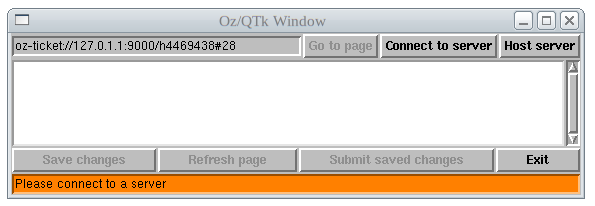
\includegraphics[scale=0.5]{connection.png}
		\caption{L'application en phase de connection}
	\end{figure}
	\begin{figure}[h]
		\centering
		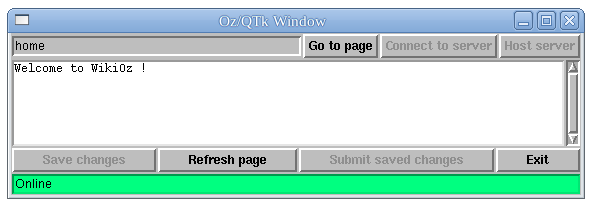
\includegraphics[scale=0.5]{connected.png}
		\caption{L'application en phase de navigation}
	\end{figure}
	
	\subsection{Se connecter au réseau}
	La première étape lorsque l'on ouvre le programme est de se connecter
	à un réseau pair à pair. Notre implémentation permet à l'utilisateur de
	choisir deux options. 
	
	\emph{Host Server} initialise un nouveau réseau
	pair à pair avec un nombre suffisants de noeuds pour que celui ci puisse
	fonctionner correctement. Ensuite, l'application s'y connecte et renvoie
	à l'utilisateur un ticket oz pour que d'autres applications puissent s'y
	connecter. Dans ce cas l'ensemble du réseau pair à pair tourne dans
	un seul processus.
	
	\emph{Connect to Server} se connecte à un réseau pair à pair existant.
	Pour ce faire, l'utilisateur doit disposer d'un ticket oz. Si un serveur
	tourne déjà sous le même utilisateur Unix, alors l'application ira
	automatiquement chercher le ticket dans un fichier se trouvant dans
	le répertoire utilisateur. Sinon, l'utilisateur devra trouver son ticket
	oz par mail ou sur un site web. 
	
	Une fois connecté, l'utilisateur peut en appellant \emph{Host Server}
	récupérer un ticket oz vers son client pour que d'autres utilisateurs
	puissent se connecter au réseau via sa machine. 
	
	\subsection{Navigation des pages web}
	Une fois connecté à un réseau, l'utilisateur entre sur la page par défaut
	\emph{home}. L'utilisateur peut se rendre sur n'importe quelle page en
	entrant son url dans la barre du haut. Si cette page n'existe pas, 
	une nouvelle sera automatiquement créée. l'url n'a pas de format spécifique
	et peut être n'importe quelle string. 
	
	L'utilisateur peut aussi rafraichir une page ce qui lui permet d'accéder
	à la dernière version.
	
	\subsection{Édition des pages web}
	Lorsque l'utilisateur est sur une page, il peut la modifier à loisir.
	Pour cela il suffit de l'editer. Après chaque changement dans un paragraphe,
	l'utilisateur doit les sauvegarder. Une fois tous ses changements
	effectués et sauvegardés il peut les envoyer sur le réseau. En cas
	de conflit dans un paragraphe, les changements ne sont pas effectués,
	l'utilisateur est notifié, et la page est rafraichie à sa version la plus
	récente. 
	
	\section{Validation des requis}
	Les deux tests présentés ci-après montrent la gestion des différentes modifications,
	lors d'un conflit et lors d'une modification concurrente réussie.
	
	\subsection{Gestion d'un conflit d'édition}
	Le plus simple cas pour réaliser un conflit d'édition est de suivre les étapes suivantes:
	\begin{itemize}
		\item Démarrer un premier client
		\item Démarrer l'anneau de noeuds ''server'' sur un des deux clients.
		\item Démarrer un deuxième client et se connecter au premier.  Par défaut, le ticket
			du premier sera déjà dans la barre d'adresse.
		\item Sur le premier client, modifier la ligne de texte, sauvegarder et soumettre les
			changements.
		\item 	
	\end{itemize}
	
	\subsection{Gestion de modifications concurrentes indépendantes}
	
	\section{Architecture}
	
	\section{Design}
	
	\subsection{Limitations}
	Notre application actuelle est sympathique en tant que proof-of-concept,
	mais souffre d'un certain nombre de limitations.
	\subsubsection{Connectivité} 
		Pour l'instant, pour se connecter, l'utilisateur doit posséder
		un ticket oz vers le processus ayant instancié le réseau.
		Si jamais ce processus n'existe plus il sera impossible pour de
		nouveaux clients de se connecter au réseau. 
		
		Pour résoudre ce problème il faudrait que chaque client puisse
		générer un ticket à partir duquel l'on puisse se connecter.
		
	 \subsubsection{Modifications Concurrentes}
	 	Si l'algorithme de merge du format symbolique des pages est
	 	assez intelligent, l'algorithme qui génère ce format symbolique
	 	ne l'est pas suffisemment. 
	 	
	 	Les conséquences sont qu'il faut enregistrer localement à 
	 	chaque modification de facon manuelle, qu'il ne peut y avoir qu'une modification par
	 	paragraphe, et qu'on ne peut supprimer qu'un seul paragraphe par
	 	transaction. 
	 	
	 	Pour résoudre ces problèmes, il faudrait garder une copie de
	 	la version originale aux cotés de la version modifiée par l'utilisateur.
	 	Cela permettrait de ne pas devoir augmenter les numéros de versions
	 	de paragraphe à chaque modification, et la sauvegarde locale peut
	 	se faire automatiquement, ce qui rendrait l'utilisation de notre
	 	programme plus conviviale. 
	 	
	 	Un autre souci est la gestion des conflits de transaction.
	 	Pour l'instant les changements sont annulés. Il serait plus
	 	intéressant de renvoyer une version contenant les conflits à résoudre
	 	comme le font les Systêmes de contrôle de versions.
\end{document}
